\scanpage{75}
% archive sheet number: 74
% @ L1–3
Mais les circuits plus généraux \deleted{\unsure{restent|restent-ils}} mystérieux pour moi -- je ne sais s'ils sont \unsure{bitables|bistables|bi-stables|valables} !

% @ L4–13
Les deux procédés correspondent à la $=$ structure polygonale sur l'\unsure{ens|un|ens.} des arcs de spécialisation \inserted{(= transition)} pour une pos. stable $D$ -- mais il y a une autre structure polygonale, due au fait que les \deleted{\unsure{uns des|arcs des}} arcs de spécialisation \uline{sur $D$} (au lieu de $\widetilde D$) sont naturellement disjoints, donc on peut prendre la structure polygonale correspondante, dont la réalisation top. est enc. $D$ lui-$=$. L'ennui, c'est que cette fois on a un polygône \deleted{\unsure{d'ordre algébrique}} \inserted{d'ordre $n$} non $2n$, \deleted{\unsure{dt|dont}} dont la signification géométrique des disques angulaires correspondants n'est pas claire. Mais peut-être est-ce une indication pour attacher \uline{simultanément} \uline{de deux façons} antipodiquement les disques $\Delta^*_{D},\Delta^*_{D'}$, de façon à obtenir un ruban de Möbius peut-être ?

% @ R1–6, with a lens-shaped drawing inside the sentence
L'idée maintenant, c'est de prendre la découpe de $X$ suivant la partie

\figure{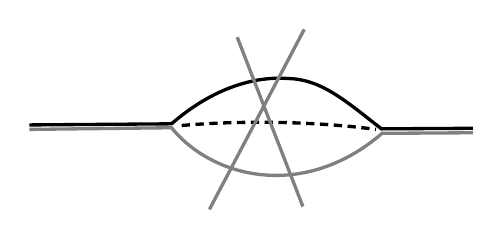
\begin{tikzpicture}[x=.86cm,y=.71cm]
\draw[very thick] (-3.5,0)--(-1.4,.02)..controls(-.85,.6)and(-.24,.88)..(.32,.83)..controls(.81,.82)and(1.17,.43)..(1.7,-.07)--(3.05,-.06);
\draw[gray,very thick] (-3.5,-.08)--(-1.4,-.05)..controls(-.8,-.95)and(.55,-1.36)..(1.71,-.15)--(3.05,-.14);
\draw[very thick,densely dashed] (-1.25,-.01)..controls(-.2,.1)and(.88,.04)..(1.62,-.08);
\draw[gray,very thick] (-.43,1.57)--(.54,-1.46) (.56,1.71)--(-.84,-1.51);
\end{tikzpicture}}

% @ R6–11 and notes within the lines
commune de $D$ et $D'$ (cf figure) ça donne donc un ruban de Möbius, \deleted{qu'on peut obtenir} \inserted{découpé par la ligne} pointillée en une bande rectangulaire. On prend le revêtement \deleted{\unsure{des}} \inserted{des orientations d'}ordre 2 du ruban de Möbius, \margin{(twisté par $\underline\omega(D)$ ?)} qui est formé de deux rectangles \unsure{vrillés|recollés} en 2 paires d'arêtes.

% @ R12–20
Sauf erreur, c'est l'identification \deleted{de} simultanée de \deleted{\unsure{$a'$|$a$}}\inserted{$a$} avec $b$, \deleted{\unsure{de|et}} \deleted{\unsure{$a$|$a'$}}\inserted{$a'$} avec $b'$, suivant le transport parallèle. Mais ce qu'on obtient, en faisant tous ces recollements pour l'ens. de tous les $\Delta_D^*$, est-elle bien la surface cellulaire obtenue par le graphe $\Gamma_{\unsure{\mathscr K|K|\Sigma}}$ et sa structure de polygonalisation et de transport ?, obtenue
